\part{Performance Analysis}

\chapter{Performance Analisys Introduction} \label{analysis-introduction}
\emph{"Every database vendor cites benchmark data that proves its database is the fastest, and each vendor chooses the benchmark test that presents its product in the most favorable light"}\cite{burleson}.

In this chapter we will introduce the database performance analysis' problem, and so we will discuss about how to measure the performance, how to understand which is the fastest and how to choose the best database depending on your needs. This preface is not specific to in-memory databases, but can be generalized for every DBMS.
	
	\section{Impartiality Problem}
The most important problem related to performance analysis, and benchmarking, is the validity, understood as impartiality, of the results. It's impossible to develop a benchmark which produces the same results obtained by real applications, and it's very hard to have the results similar to real performance too. Moreover every benchmark may produce valid results only for a small set of applications, and therefore there is the need to use different benchmarks. All these difficulties were emphasized by vendors who, with benchmarks wars and benchmarketing, complained for fake results, and consequently brought to a lack of trust in benchmarks. In this section we discuss about these difficulties, starting from a benchmark's definition until an analysis of the main differences in benchmarks which produce different results.

		\subsection{Benchmark Introduction}
Before starting all this discussion, it's necessary to explain the benchmark's meaning in computer science. The term benchmark refers to the act of running a program, or a set of programs, against an object in order to evaluate its performance, but it is also mostly used to represent the program or programs themselves. In this work we refer to software benchmarks run against database management systems. The main purpose of a benchmark is to compare the performance of different systems across different platforms. With the advance of computer architecture, it is become more difficult to evaluate system's performance only by reading its specifications. Therefore a suite of tests is developed to compare different architecture. This suite of tests, intended as validation suite, is also used to verify the correctness, the properties of a software. 

In particular benchmarks mimics specific workload giving a good measure of real world performance. But ideally a benchmark should substitute the application simulated only if it is unavailable, because only the real application can show real performance. Moreover when performance is critical, the only benchmark that matters is the inteded workload.

The benchmark's world is full of challenges starting from a benchmark development, to the interpretetion of the results. Famous benchmark tend to become useless after some time, because the vendors tune their products specifically for that benchmark. In addition most benchmarks focus only on the speed which is expressed in term of throughput, and forget many other important features. Moreover many server architectures degrade drastically near 100\% level of usage, and this is a problem which is not always taken into consideration. Some vendor may publish benchmarks at continuous at about 80\% usage, and, on the other hand, some other benchmark doesn't take this problem into account, and execute only tests at 100\% usage.
		
		\subsection{Benchmark History} \label{bench-history}
As already highlighted in the previous paragraph, with the advance of computer architecture the performance analisys became more difficult: it's not possible to evaluate a system only by reading its specifications. A computer program, a benchmark, simulating a specific workload, became a solution to this problem.

The first benchmarks were developed internally by each vendor to compare their database's performance against the competitors. But when these results were published, they weren't considered reliable, because there was an evident conflict of interest between the vendor and its database \cite{gray}. This problem was not solved by a benchmark pubblication by a third party, which usually brought to a benchmark war.
	
		\subsubsection{Benchmark Wars}
Also when benchmarks were published by third parties, or even by other competitors, the results were always discredited by losing vendors, who complained for the numbers, starting often a benchmark war. A benchmark war started when a loser of an important and visible benchmark reran it using specific enhancements for that particular test, making them get winning numbers. Then the opponent vendor again reran the test using better enhancements made by a "one-star" guru. And so on to "five-star" gurus. Every result so obtained by a benchmark could not be considered a valid result, firstly because the vendors themselves don't give any credit to the result, secondly because the result, with its relative numbers, changes too much frequently. 

		\subsubsection{Benchmarketing}
Benchmarketing is a variation of benchmark wars. Due to domain-specific benchmarks there was always a benchmark which rated a particular system the best. Such benchmarks may perform only a specific operation promoting one database instead than others. For example a test may execute only one type of transaction, or more reads than writes and therefore promote an in-memory database over a traditional DBMS. To summarize, a benchmark may simulate different scenarios favouring a particular database. Therefore each vendor promotes only the benchmarks which highlight the strengths of their product, trying to impose them as a standard. This leaded to a ploriferation of confuse benchmarks and didn't bring any benefit to the benchmark's reputation.

		\vspace{0.5cm}
Although these phenomenons were drastically reduced by the foundation of the Transaction Processing Performance Council (TPC) in 1988, they are still alive nowday.

		\subsection{Benchmark Differences} \label{categories}
It is now evident how hard is to understand which database is the fastest. Benchmarks cannot be properly used to analyze the performance of several databases and choose simply the best. Every benchmark has a bias, testing some particular aspect of database systems, such as writes, reads, transactions and so on. Moreover every benchmark operation can be implemented in different ways by the same database: creating a connection for every operation or using a connection pool; use different transaction isolation level; load the whole database in RAM or split it in different hard disk partition; etc. Furthermore the same benchmark, with the same implemention for every database, can show dissimilar results when it runs on different platforms (hardware and software).

All these differences are grouped by three categories:
\begin{enumerate}
	\item Test scenario: reads, writes, etc.
	\item Test implementation: there are different way to implement the same transaction.
	\item Execution platform.
\end{enumerate}
	
		\subsection{The Axiom}
By this reasoning comes out the axiom which will guide the following chapters, and the work behind this thesis:

\label{axiom} \emph{"There is not a slower or a faster database: databases are only slower or faster given a specific set of criteria in a given benchmark"}.

This sentence comes from an article by Bernt Johnsen \cite{Bernt}, who, in response to a benchmark comparing HSQL and Derby, stated that it's easy to make a benchmark, but it is always hard to communicate the meaning of the results. The interpretation depends on too many criteria, so that it's not easy to say which database is the fastest, unless specifying the set of criteria used in the benchmark.
	
		\section{Measures}\label{measures}
Even if we cannot state which database is the best by analyzing their performances on standard benchmarks, we can still measure other parameters that can be later interpreted to choose the database system which best fit our needs.

When choosing a database, the most important features to evaluate and compare are:

\begin{description}

	\item[Throughput]: is the number of transactions per second a database can sustain. This is the most important feature to consider when evaluating a database system. The most representative application scenario to understand the meaning of the throughput is an on-line transaction processing system. This kind of application requires the database to sustain a certain number of transactions per second, based on the number of users, and not every database can suite the needs of the application itself. Another example is real time applications: they require even higher throughput as well as very low latencies. Therefore it is crucial to understand if a certain database is suitable for an application in terms of transactions per second.
	
	\item[Latency/responsiveness]: is the time the database takes to execute a single transaction. This is the most important parameter in real application where the response time is a vital feature. In some case, where transactions are executed synchronizedly by a single user, latency can be measured as the inverse of throughput.
	
	\item[CPU load]: is the average percentage of the CPU processing time used by the database. It becomes an even more important parameter when the database is not the only service running on a server. CPU is a precious and limited resource, shared by all processes in a particular machine, and although database systems are usually deployed on dedicated servers, embedded databases live collated with the application that uses them. Many in-memory database 	don't even have a "stand aone" version and are mainly used as embedded db.
	
	\item[Disk I/O]: is the measure of the amount of data transferred to and from the disk. It is often a bottleneck for every traditional databases. Altought pure in-memory databases never access to the disk, when adding durability through a transaction log file, disk I/O is a bottleneck for IMDBs too. This parameter could be considered less important since all databases will incure in the same performance bottleneck, but it is possible that different DB coudl use the disk in different ways and suffer more or less impacts from it.
	
	\item[File size]: is the size of the database image on the hard disk. While traditional DBMS' store objects (tables), indexes and a transaction log file on the file system, in-memory databases usually store only a journal file containing all the transaction executed on the database. Altought this may seem a small file, it can become very huge, even more than the database image. This measure is interesting whereas each database use different data structures.
	
	\item[RAM usage]: is the quantity of RAM a process uses while running. Talking about in-memory database, this can be another way to measure the size of the database image. In addition, this is a critical value to take in mind: IMDBs only works correctly and efficiently under the hypothesis that the RAM is enough to contain the whole database. Therefore this can be an important parameter to take into consideration when deciding if a DBMS fits your requirements.
		
	\item[Startup time] is the time the database needs to become operational. This is a very important parameters for applications which need high availability, and in this case the startup time plays a crucial role to respect the maximum time the application can be off-line or not completely operative. 
	
	\item[Shutdown time] is the time the database takes to shut down and kill the process.
	
\end{description}
	
	\section{Choosing a Database}
From the previous sections, it's now clear how difficult it is to use benchmarks to prove which database is the fastest. Even with a fair benchmark, which can be very useful to understand the performance of databases, it is still difficult to choose a database: performance is only one factor to consider when evaluating a database \cite{burleson}. 

Other factors to consider are:
\begin{itemize}
	\item The cost of ownership.
	\item The availability of trained DBAs.
	\item The vendor's technical support.	
	\item The hardware on which the database will be deployed.
	\item The operating system which will support the database.
\end{itemize}

In other words, it is very difficult to choose the right database for our needs, and, of course, while evaluating databases and benchmarks there is absolutely \emph{no winner}.

For this reason, what we will introduce in the next chapter is a suite of tests which has been developed with these concepts in mind. What we tries to achieve is a way for people to judge, analyze, verify and evaluate any DBMS (especially in-memory databases) with a chance of developing their own set of test and run the test suite on any hardware and under (virtaully) any operating system. The application is Java-based and so it ansures the widest coverage of both hardware and operating systems.


\chapter{Test Suite} \label{test-suite}	
In this chapter we are going to discuss the first of the three big differences, described in paragraph \ref{categories}, which make a database faster or slower: the test scenarios used to run a benchmark and to analyze database's performance. These test scenarios will be used to build test cases, a collection of different scenarios, one or more, executed concurrently. All these test cases will compose the test suite we are going to use for database benchmarking. Therefore in this chapter besides a tests' description, a suite of test will be created, allowing us to analyze the databases' features of our interest. 

The tests are divided into three categories: base test case, load test case and acid test case. The first category contains simple tests configured as a race between databases, and it is used to obtain an approximate idea in an early stage. Instead, the second category simulate real application scenario, and it can give us a detailed analysis of the real database's performance. Finally the last category is built to understand if the database is ACID compliant.


	\section{Why Define Test Scenarios}
The axiom, previously described in paragraph \ref{axiom} at page \pageref{axiom}, expresses clearly the difficulty to analyze databases' performance and how every result obtained in a given benchmark depends on the specific set of criteria used in the benchmark itself. In paragraph \ref{categories} there is also a description of the three major categories in which the criteria fall. The first of these categories is test scenarios: different test scenarios may show completely different performance results. It's not possible to avoid this behavior, but we can define clearly every tests so that we will be aware of the differences between them. 

Moreover we can model these tests in a way they simulate real application scenarios, so that real performances will be very close to the results obtained by the tests.

	\section{Base Test Case}
Base test case is a collection of very simple tests, which are configured mostly as a race. This is exactly what the majority of benchmarks does, particularly Poleposition \cite{poleposition}.

Every test can execute different read/write operations on the database, such operations are grouped into \emph{tasks}. The word \emph{task}, used extensively in the following paragraphs, refers to a collection of operations. Each task is then repeated, and since all the operations in a task are synchronized and executed consecutively, the number of \emph{task per second} is the same of the \emph{transaction per second} of each operation involved by the same task. Therefore \emph{task, or task per second} and \emph{transaction, or transaction per second} can be used in this contest without any distinction, and they all refer to the operations' \emph{iteration}.

The key features of these kind of test are:
\begin{itemize}
	\item A fixed number of tasks' iteration before the test stops: so tests are configured as a race where every database must execute a certain number of transaction.
	\item A fixed amount of time before the test stop: as an alternative to a fixed number of transaction, every test run for a specific amount of time, executing the maximum number of iteration. 
	\item Different kinds of objects: tests must be able to create/retrieve/update/delete simple flat objects with few fields, or complex flat objects with many fields, or still hierarchical objects, and so on. This feature let us test effectively the performance on the objects used in the domain of our interest.
	\item Single task: to keep these test simple it's better to avoid concurrent tests, but it is still possible to implement concurrently the different operation executed on the database.%dubbio sulla concorrenza
\end{itemize}
	
		\subsection{Race Test: Timed}
We already said base tests are configured inherently as a race. These tests can be used to show the maximum throughput the database can reach doing a particular operation on a specific object. Metaphorically it's like a rocket car in the desert trying to reach its speed limit. In a real application this is rarely useful, but can give us an idea of the database's limits. 

In order to create a test scenario we have to define the domain object/s involved in the test, the operations on which the test loop and when the test should stop. For example:
\begin{itemize}
	\item The object represent a person, with only two fields: an id number and a name. This is a simple flat object. 
	\item The only operation executed by the test is a write operation: every time an object will be added to the database.
	\item 60 seconds is the stop condition of the test: after 60 seconds of iteration of writes (objects person inserted in the database) the test stops.
\end{itemize}
Clearly the time is not a significant measure, every test's execution run for the same amount of time: 60 seconds. Instead of the time, a more interesting measure to take is the throughput. This test shows the maximum theoretical value for the throughput, which in a real usage scenario will never be outperformed. 

This test, and its results, are not useful to understand the real performance and potentiality of the database and so they are not useful to choose the database for our needs, but it can be used in an early stage to reduce the databases' set which will be analyzed extensively with further tests. In other words we can throw away every databases whose maximum throughput is not enough for our needs.

		\subsection{Race Test: Transactions}
This test is really similar to the previous test. The only difference is in the stop condition:
\begin{itemize}
	\item The object represent a person, with only two fields: an id number and a name. This is a simple flat object (same as before). 
	\item The only operation executed by the test is a write operation: every time an object will be added to the database (same as before).
	\item 1.000.000 of iteration is the stop condition of the test: when 1.000.000 of writes are executed (objects person inserted in the database) the test stops.
\end{itemize}
While in the previous test the duration was meaningless, this time, like in a race, it shows which database is the fastest (the winner of the race). Despite this, the duration is still of little use. Also for the throughput the same considerations made before are still valid.

But this new test is useful also to take other interesting measures, such as the file size, which, as explained in par. \ref{measures}, can become very huge, even more than the database image, and therefore it is a critical measure. We can evaluate how the file size increase with the number of objects (person) inserted in the database. This is because, differently to the previous one, every test's execution perform a fixed amount of iteration. 

	\section{Load Test Case} \label{load-test-case}
Restrictions introduced by base tests are very simple to read and they can be useful for a first look and for fast and approximate results. These restrictions are due to the impossibility to simulate real complex application scenarios. Substantially the main restrictions are:
\begin{enumerate}
	\item Real application scenario are rarely single thread/task: to stick to the axiom at paragraph \ref{axiom}, the best way to understand which database fits our needs is to make test scenarios as much realistic as possible.
	\item The second restriction is a direct result of the first: trying to make test scenarios more realistic, it is necessary to introduce some sort of control for the throughput. When a test stress the database engine to its maximum level, some other mechanisms may not work properly, such as the garbage collector, caching, indexing, etc. In addition, when a test concurrently accesses the database, this restriction is even more evident: if a thread is not limited in its transactions per second, it will impact the performances of other threads, not to mention the locking that will occur on the DB.
\end{enumerate}

Base test case offer very important and useful results, but when it comes to test the average load of a real application of our interest, they are not enough. These restrictions are solved by load test case, which allow a better simulation of the application scenario. The key features of these tests are:
\begin{itemize}
	\item Multi-tasking: different task, and therefore different sets of operations, can be executed concurrently against the database.
	\item A bond on the throughput: in order to simulate real application usage, for every task it is possible to specify the maximum throughput in terms of iteration per second, if the database can reach it.
\end{itemize}

From these features comes the name "load test case", which means the simulation of an average, or specific, load on a certain database. This idea, and the need of this kind of tests,  can simply be exaplined by a Bernt's metaphor, who has been already cited for the axiom at paragraph \ref{axiom}. The metaphor is:

\emph{"I don't buy the fastest car in the market. I don't even buy the fastest car I can afford. I buy a car I can afford that fits my needs... e.g. drive to the northern Norway with 2 grown-ups, 3 kids, a kayak, sleeping bags, a large tent, glacier climbing equipment, food, clothes and so on. Can't do that with a Lamborghini"}\cite{Bernt}.

This metaphor explain exactly the need not for the fastest database, but for a database which can sustain the load of the application without any complexity during its normal functioning, such as a database snapshot freezing all writes operation, or a bug/memory leak making the database crash.

		\subsection{Real Time Prepaid System} \label{real-time-test-case}
Keeping these features in mind, we want to create a load test case to analyze exactly which performance  a database system  offers for a practical use case: a real time prepaid system, such as a telephone company. Basically the test is the concurrent execution of 3 different task, each simulating complex scenarios: services authorization and management, balance checks and accounts management.

We start describing the domain objects used by this test, and then we move on to the analysis of the different tasks involved.
		
			\subsubsection{Domain Objects}
Domain objects involved by this test are typical for a telephone company who handle telephone calls for every person, which is rappresented by an account, and which can access to many service through a web application, offered by the company for its customers. There are four domain objects used byt this test:
\begin{description}
	\item[Account]: this object represent a customer in the real time prepaid system. It contains all the typical information needed by a telephone company, such as the balance, the type of subscription, etc. In other words, this is a complex flat object, that has many private fields but no hierarchies. In a real application there are millions of accounts instantiated in the database, one for every customer. This dimension is also very important to make the simulation as real as possible, in order to get realistic results.
	\item[MSISDN]: it is the unique number which identify a subscriber in a GSM or UMTS mobile network, it is the telephone number. Each msisdn object is linked to an account. Therefore there are also millions of MSISDN objects in the database, referring to a real application.
	\item[Webuser]: this represents the customer logged in the company web site. It contains the username and the password to access to web services. In common with MSISDN, it is linked to an account too, and both are simple flat objects: a very simple object with few fields.
	\item[Session]: when a customer start a call, an object session is created, and it keep all the information about the call which is going on, until the call ends. After the call this object is deleted. A session contains the start time of the call, the time of the last unit and all the relevant information for the authorization process to take place. Each session references to an account, the one who started the call. But there are not as many sessions as accounts, not everyone will start a call at the same time, except New Year's Day! A reasonable size for the session objects is the number of hundreds of thousands concurrently going on.
\end{description}

			\subsubsection{Balance Check Task}
This task simulate a customer checking his residual balance for the prepaid card, a SIM in the case of the telephone company. First, the customer logins in the website or calls the dedicated number, and then receives all the details on his balance.

Each task, as already explained, corresponds to a transaction composed of different operations. This leads to illustrate how the task work in terms of operations executed:
\begin{enumerate}
	\item \emph{Read} randomly the MSISDN if the customer makes a call or the webuser if he access to the website.
	\item \emph{Read} the account referenced by the MSISDN or webuser, and then check the residual balance, a simple account's field.
\end{enumerate}
So this task executes a total of two read for every iteration.

Another important parameter to make this task a part of a load test is the amount of transactions per second this task should sustain. The average throughput for check balance task, considering there are millions of accounts in the database, is about ten transactions per second.

			\subsubsection{Accounts Management Task}
The account management task simulates the subscription of new customers and consists pf the creation of an account object and the relative MSISDN and webuser.

The operations involved by this task are:
\begin{enumerate}
	\item \emph{Write} of a new account: all informations of a customer are inserted in the system by creating a new account object.
	\item \emph{Write} of a new MSISDN, containing the telephone number of the new subscriber.
	\item \emph{Write} of a new webuser with username and password for the customer.
\end{enumerate}
To sum up, this task executes three writes on the database for every iteration.

To simulate a real scenario, the average throughput is about ten transactions per second.

			\subsubsection{Services Authorization and Management Task}
This task simulates a call started by a customer. After checking the balance, and therefore if the account is allowed to start a call or use a service, a new session is created and updated every 30 seconds, the unit time. On the average a call lasts about two minutes. When a call ends the session is deleted.

In terms of operations executed on the database, it can be described as follow:
\begin{enumerate}
	\item \emph{Read} the MSISDN of the customer starting the call.
	\item \emph{Read} the account referenced by the MSISDN, and its residual balance, and the other parameters, to check the user's permissions for the service requested.
	\item \emph{Write} a new object session and \emph{update} account's balance.
	\item \emph{Update} the session every 30 seconds and the account's balance.
	\item \emph{Delete} the session after the call is ended.
\end{enumerate}

This is the most complex and important task, because it represents a very frequent task. No wonder if the average throughput is about 2000 transactions per second.

			\subsubsection{Real Time Prepaid System Summary}
To sum up this whole load test we have to define the objects used by the test, the task concurrently executed, and when the test stop.

There are four domain objects involved by this test. Three of these are simple flat objects (objects with few private fields): MSISDN, webuser and session. The forth is a complex flat object (objects with many private fields): account. To test the system in its normal operational scenario we will have the system preloaded by some millions of objects before starting the actual test.

Three task are executed concurrently. One is the major task, simulating a customer's call, and it runs 2000 times per second. This task is the bottleneck of a real application, and it could be also tested alone in a base test to understand the database's limits in running this task, and therefore to have an idea of the database potentiality. The other two are secondary tasks, in fact the throughput is limited to ten transactions per second.

This test is a load test and therefore we are not interested in stopping it after a certain amount of transactions executed. But what we want is to let the test run for many minutes until to many hours to understand if the database can sustain the load generated by the test.
			
	\section{Acid Test Case}
Base and load test case are used to analyze databases' performance, but, as already said, a database is not made only by performance: there are many other parameters to take into consideration before judging a database, such as ACID properties. To make these tests an all-round test suite, we could add some tests for verifying databases' ACID properties. The above corresponds to the work done by the Transaction Processing Performance Council with their TPC-C benchmark \cite{TPC-C}: \emph{performance is not the only benchmark's goal, but ACID properties are tested too}.

Especially the durability property is most interesting to analyze when talking about in-memory databases. Pure IMDB have no durability at all, while it can be added in different degree, as already described in paragraph \ref{durability}. Therefore would be very useful to know how strong is the durability solution implemented by the in-memory database, although listening to vendors' words their database management systems should offer always strong durability.

Nevertheless, testing ACID properties is not a simple goal to achieve. Particularly the durability is the hardest property to be tested. Also the tests developed by TPC are not intended to be an \emph{exhaustive quality assurance test}.
%Citazione tpc pdf pagina 46 \cite{TPC-C}

\chapter{Database Benchmark Softwares Overview} \label{overview}
The difficulty to analyze objectively databases' performance has already been exapalined and understood in chapter \ref{analysis-introduction}. The major problems were found in the differences of test scenarios, implementation and execution platform. In the previous chapter we tried to minimize the first issue by modeling different test scenarios like real application scenarios. This is not a panacea, but in this way results produced by these tests are more valid for the applications they simulate than generic tests. 

The focus is now moved on the second and third issues: the tests' implementation and the execution platform, in other words an application benchmark used to run test scenarios. In this chapter we analyze more or less deeply different open source benchmarks trying to find a benchmark for our needs, or, in the case it's not suitable, to take some idea for a future development of a new benchmark application.

	\section{Benchmark Requirements} \label{requirements}
Before starting the analysis, it's necessary to make clear the requirements a benchmark should have to run our tests. These requirements will give us a set of parameters which can be used to evaluate properly a benchmark. But before stating all the requirements, it's important to point out some general characteristics for a benchmark:
\begin{itemize}
	\item Not only a single metric: a benchmark should show the results with different metrics in order to provide a better awareness of the results themselves.
	\item \emph{The more general the benchmark, then less useful it is for anything in particular}: it's impossible to make a benchmark for everything, it's better to put some limitations and produce proper results for a specific task.
	\item Based on a workload: only the essential attributes of a workload should be used to create a benchmark.
\end{itemize}
  
These general characteristics and some of the following requirements are taken by the TPC presentation at the sigmoid conference in 1997 \cite{tpc/sigmoid}, a bit old work, but this council is still active and of course they know how to make a benchmark.

The requirements we are going to analyze are: portability, understandability, flexibility, detailed report, visual report, both for relational and object databases and easy to use. In addition we will illustrate some benefits a benchmark should bring. 

		\subsection{Portability}
A benchmark is a set of tests runned against a system, a database in this case, to analyze the performance with the main purpose to compare them. The comparison is usually between different systems when you are choosing the best in term of performance for your needs. But when you already have chosen the system it is also very useful to compare the benchmark's results on the same database between different platform. In order to make this possible, both the system to be tested and the benchmark must be able to run on several platforms. While databases usually run on different operating systems, it's not the same for benchmarks. When the benchmark runs on a client's network, and therefore it is for client-server databases, it can be considered portable, because the execution platform doesn't matter. But when we are using embedded databases, the benchmark itself must live togheter with the database system, and therefore able to run on different OS, which means it is portable.

Thus, when testing embedded databases too, a portable benchmark can help us not only in the decision of the best database system given a certain platform, but also in choosing a suitable platform for our database.

		\subsection{Understandability}
This feature may seem obvious, but it is not when we are reading thousands of incomprehensible words or graphs with many lines and no legends or captions on the axis. The capability of being understood is essential to make the benchmark useful. Understandability is intended in terms of clear results and their easy interpretation:  as already explained in paragraph \ref{bench-history} benchmarks' results are easy to be tricked and cheated, and therefore they must be clear to avoid any religion's war and consequently the distortion of the results. 

Moreover, it's important to take in mind there are different stakeholders interested in benchmarks' results: engineers working at the database engine, managers selling the system and customers interested in buying a database. Thus a good benchmark must be able to be easily understood by many people and provide a clear view or views of the results.

		\subsection{Flexibility} \label{flexibility}
This is not a requirement for every benchmark, but it is for our purpose. We want a benchmark which can run the test suite described in chapter \ref{test-suite}. That is the collection of tests we gathered and we want to run against a database system to understand its performance. Therefore we need a benchmark which with few programming can execute our tests. 

Furthermore, recalling the axiom in paragraph \ref{axiom}, benchmarks' results may depend on too many criteria, and therefore a good benchmark must be flexible in order to simulate the real application scenarios we are interested in, scenarios which we may add in the future. Although we said in this paragraph's introduction a benchmark should not be general because it becomes less useful, it is also true that a good benchmark must be based on a workload, the workload of the application which will use the database system we are going to choose. Therefore flexibility is a key feature for a benchmark when comes the need to run a own test suite based on the workload of our application.
		
		\subsection{Detailed Report}
Recalling the first general feature for a benchmark in the introduction of this paragraph ("not only a single metric"), results must provide different measures allowing a better understanding of databases' performance. It's not by chance we are talking about understandability. These two characteristics are strictly connected. Of course many measures for every test will make the result harder to understand but will provide more informations to interpret the databases' behavior. On the other hand only one measure is easier to understand but may hide the database behavior and the reasons behind that. Therefore a compromise is needed: in each test we are not interested in all the measures it's possible to take, but only a subset of those can be taken for every test. The reference measurements have been already introduced in paragraph \ref{measures} and they represent a subset of all possible measures for a database.

In addition more measures the benchmark's application takes, more it alters the database performance, and therefore a compromise in the number of measures is always a good choice, but keeping in mind that only one measure will not tell much about databases performance.

		\subsection{Visual Report}
In order to make the results even more understable, and to make the detailed measures more readable, visual reports will play an essential role. Graphs are able to express thousands of numbers in one or few colored lines. Graphs are perfect not only to show the final result of a test, but also the whole trend, from the beginning to the end. Therefore any oscillation in the measures can become evident and easy to read. It will not be hide by an average value reported at the test's end. Of course graph can also be almost useless if they report only the final value. It depends by the implementation. For example graphs such as those from Poleposition benchmark, which will be analyzed in paragraph \ref{poleposition}, may be very hard to understand and they simply describe an average value.

Furthermore visual reports are usually used with the main purpose to compare system between them, and this is another task they play perfectly. Of course there are many parameters to understand before being able to read properly a graph, but then in a simple graph every line can represent a different database system, allowing an easy comparison between them. This is really appreciated by non technical people, such as managers or customers. For this purpose graphs are a must, and therefore this is a feature we want from a benchmark application.

		\subsection{Both Relational and Object Database}
The benchmark we are looking for must be able to work with both relational and object databases. Relational databases are usually able to run as stand-alone server and accessed via SQL. Instead object databases are used mainly as embedded databases and accessed via a native interface for a specific programming language. Anyway in-memory databases are used mainly as embedded databases and therefore we need a benchmark which can use embedded databases accessed by both SQL (eg: JDBC) and native interface. Although in-memory databases are not a new technology, they became widely used in the last few years, therefore many benchmarks do not provide any support for embedded databases.

When testing both relational and object databases another problem comes out: the benchmark application can test the database systems in different ways, using a relational point of view or an object oriented point of view, or both. This may produce different results in the performance analysis. The knowledge of this feature is important during the results' analysis.

		\subsection{Easy to Use}
This is a commonplace for every application, nobody wants something impossible to use. As for other requirements, a compromise is always needed, especially for this feature. The ease of use, in this case, means the possibility to modify several test's parameters, such as the parameters already explained in chapter \ref{test-suite}, and also to be able to bring some little variation to the workload simulated, in order to improve the test when the needs change. This ease of use, understood as a variation in parameters, should be granted without any modification in the application's lines of code, but for example in an xml file, or other configuration files, or with some input parameters.

Of course this may seem similar to the flexibility requirement, that we discussed in paragraph \ref{flexibility}, but while flexibility is intended as the capability for engineers to implement completely new test scenarios, ease of use is the capability to execute the workloads implemented with few variations, such as the initial database's state, the exact operations' order, etc. This requirement is needed for all the non technical people who want to analyze the database performance.

		\subsection{Benefits}
Discussing about requirements, it's important to note also the benefits a benchmark should bring, the aims it is built around. Referring again to the TPC presentation at the sigmoid conference in 1997 \cite{tpc/sigmoid}, the benefits a good benchmark should bring are:
\begin{itemize}
	\item Definition of the playing field: a benchmark should clearly point out the database performance and the hypothesis behind these performance.
	\item Progress's acceleration: a benchmark allow to measure the database's performance and therefore engineers are able to do a great job once an objective is measurable and repeatable.
	\item Schedule of the performance agenda: this is something also managers and customers can understand. Every release can have clearly declared its goals, such as X increment in the throughput, and it is easy to measure realese to realese progress.
\end{itemize}

The TPC work illustrate also how good benchmarks have a lifetime, because they firstly drive industry and technology forward, but when all reasonable advances have been made, benchmarks can become counter productive, encouraging artificial optimizations. But this reasoning falls down when the workload, on which the benchmark is based, changes. And the modification of the workload, from little modification to completely new implementation, is a requirement for the benchmark we are looking for.
	
	\section{The Open Source Database Benchmark}
We start now the analysis of several database benchmarks trying to understand if they are suited for our needs, or to take some idea for a future development. Discussing about these benchmarks we will illustrate advantages and disadvantages. Surfing the web and looking for databases benchmark "The Open Source Database Benchmark" is the first who comes to light. 

		\subsection{Advantages}
First of all this database benchmark is open source. All the benchmarks we will analyze are open source, therefore it sounds a bit strange to point out this feature as an advantage. But this database benchmark has so few advantages that it's good to list them all.

Instead a better feature to point out is the test suite used by this benchmark application: it is based on AS3AP, the ANSI SQL Standard Scalable and Portable benchmark. This is a relational query benchmark divided in two section: single-user tests and multi-user tests. Therefore this is a collection of SQL script which can be used against a database with a minimum effort in benchmark's programming. 

		\subsection{Disadvantages}
On the other hand there are several disadvantages. This project started in the beginning of 2001 and its last release is 0.21 dated at January 2006. Therefore both the latest release number and date are bad numbers: this software is outdated and it is still in alpha release. Also the AS3AP benchmark is outdated and very few information are available on the web.

From a relational point of view, this benchmark is portable, because it runs on a network client, but it is written in C language, and it is not portable from an embedded database point of view. When porting a program written in C from a platform to another, there is almost always some code's lines which need to be changed, especially when using sockets or other system calls.

In addition this benchmark is able to run only SQL script against relational database server, thus it needs a lot of programming for the procedures' implementation to test embedded/object databases. What's more we want primarily test embedded/in-memory databases and not relational database servers.

At last, another disadvantage is the lack of detailed visual reports. This benchmark works only by the command line interface and no graphs are produced. Moreover there is no direct comparison between different database systems: in order to compare two databases, manually the benchmark must be runned against them and then compare the throughput reported. There is also no comparison in the throughput's trend during the execution of the test.

		\subsection{Conclusion}
In conclusion it is clear how this database benchmark doesn't fit to our needs. Not even one requirement is completely satisfied and some of them are taken in no consideration. The reports are neither detailed or visual, and embedded in-memory databases are not supported. With a lot of programming this benchmark can also become a good one, but it's more convenient develop a completely new benchmark than extend the open source database benchmark to fit our requirements.

What we have learned from this application is very few: only the AS3AP is a nice discovery. It is an old standard SQL test suite, which can be used to understand and to learn some new kind of test, new interesting workload. But AS3AP is very old and outdated and therefore useless.
	
	\section{Transaction Processing Performance Council}
In the past years, without a standards body to supervise the testing and publishing, vendors begin to publish extraordinary marketing claims running specific benchmarks. The Transaction Processing Performance Council, TPC, is a non-profit corporation founded in 1988 by eight leading software and hardware companies in response to benchmarketing and benchmark wars. The TPC currently has 20 full members: AMD, BEA, Bull, Dell, EnterpriseDB, Fujitsu, Fujitsu Siemens, HP, Hitachi, IBM, INGRES, Intel, Microsoft, NEC, Netezza, Oracle, Sun Microsystems, Sybase, Teradata and Unisys.

The main aim of TPC was the provision of uniform benchmark tests. Therefore they, recnognizing that different types of applications have different workload, created several benchmarks. Besides the outdated benchmark which are TPC-A, B, D, R and W, there are the followings: 
\begin{itemize}
	\item TPC-App: an application server and web services benchmark. It simulates the activities of a business-to-business transactional application server operating in a 24x7 environment.
	\item TPC-C: an on-line transaction processing (OLTP) benchmark created in 1992; a complete computing environment where a population of users executes transactions against a database.
	\item TPC-E: a new on-line transaction processing workload which simulates a brokerage firm.
	\item TPC-H: a decision support benchmark. It consists of a suite of business oriented ad-hoc queries and concurrent data modifications.
\end{itemize}

		\subsection{Advantages}
Of course there are many advantages when discussing about TPC benchmarks, and above all there is the experience this consortium has accumulated in the last twenty years. Since 1988 TPC is working on benchmarks expressing how benchmark results depend on the application's workload, on the system design and implementation, including the execution platform, and on the application requirements, such as high availability or strict durability. This experience, and the big names of the members, contributed to impose TPC benchmarks as a standard, especially for OLTP performance.

Talking about standards, the most famous TPC benchmark is TPC-C, the on-line transaction processing benchmark. The scenario simulated by TPC-C is very common real application scenario, and therefore all its success. This is a moderately complex OLTP modeling a wholesale supplier managing orders, whose workload consists of five transaction types:
\begin{enumerate}
	\item New order: enter a new order  from a customer.
	\item Payment: update customer balance to reflect a payment.
	\item Delivery: deliver orders (done as a batch transaction).
	\item Order status: retrieve status of customer's most recent order.
	\item Strock level: monitor warehouse inventory.
\end{enumerate}
The benchmark take a measure of the throughput, that in TPC terms is a measure of maximum sustained system performance. It is based on the number of "new order" transactions per minute while the system is executing all the other transactions types. In addition, while running the benchmark, 90\% of each type of transaction must have a user response time less than 5 seconds, except "stock level" which is 20 seconds.

But throughput is not the only metric used by TPC, there is also a price/performance metric. The price is simply divided by the throughput and tell you how much is the cost for a transaction. It's important to note that this price is not the cost of the hardware, or another component. It include all cost dimension of the system environment: terminals, backup storage, servers, software, and three year maintenance.

TPC-C requires also transactions to be ACID (atomicity, consistency, isolation and durability) and therefore TPC included different tests to demonstrate that the ACID properties are supported and enabled during the execution of the benchmark. These tests are not intended to be exhaustive quality assurance tests. Therefore these test are a necessary condition, but not a sufficient, to demonstrate the ACID properties. In the TPC-C specification document \cite{TPC-C} there is the description of different kind of scenarios which can be used to test the acidity of the database system.

Lastly TPC doesn't work only for creating good benchmarks, but also a good process for reviewing and monitoring those benchmarks. A nice metaphor written by Kim Shanley in 1998, chief operating officer at TPC, says good benchmarks are like good laws: as Aristotle said, if the laws are not obeyed, do not constitute good government. And this is the meaning for the process reviewing and monitoring. Although this last concept about process monitoring is really important, this is not an interesting feature for the benchmark application we are looking for, simply because it doesn't regards the application itself.

		\subsection{Disadvantages}
The transaction processing performance council offer many advantages, but its benchmarks are not exempt from disadvantages. First of all TPC benchmarks are only specification and there is no implementation available: each vendor must implement its own benchmark and then the council will review and monitor the process to check if the specification are kept. Although it is possible to find some free TPC-C implementation in internet, they are all unofficial benchmarks.

In addition all the available implementations, as for the official private implementations, are for relation database only and run SQL script. Not by chance all the TPC-C specification are expressed in terms of relational data model with conventional locking scheme. But in the introduction of TPC-C specification \cite{TPC-C} it is clearly stated that it's possible to use any commercial database management system, server or file system that provides a functionally equivalent implementation. The relation terms, such as "table", "row" or "column", are used only as an example of a logical data strucuteres.

Moreover all these benchmarks have been used for high end system and for vendors who produce both hardware and database management system. Although it's possible to use a proper implementation of these benchmarks for every kind of DBMS the comparison between the official results will be almost always of few interest: because the official results regards only high end systems and because the results obtained by the proper implementation will not get any credit by the TPC consortium.

		\subsection{Conclusion}
To sum up the whole discussion about TPC benchmarks, especially TPC-C, it's evident how this is not suitable for our needs, but instead all this work can be used as an inspiration. There are different reasons why this doesn't fit the requirements previously exaplined. The council itself wrote in the TPC-C specification \cite{TPC-C} a sentence that clearly state why this is not what we are looking for:

\emph{"Benchmark results are highly dependent upon workload, specific application requirements, and systems design and implementation. Relative system performance will vary as a result of these and other factors. Therefore, TPC-C should not be used as a substitute for a specific customer application benchmarking when critical capacity planning and/or product evaluation decisions are contemplated"}.

This is an emblematic sentence and it can be considered as an extension of the axiom enunciated in paragraph \ref{axiom} where we said that performance depend on a huge number of criteria. The meaning of this sentence is that TPC-C is a good benchmark used to compare different systems for a generic purpose OLTP, without critical performance requirements. In this case, you need a benchmark which simulates the workload of your application, or the application itself. While TPC benchmarks are not flexible, they can't be used to run our test scenarios. In fact TPC-C benchmark is simply a complex application scenario, a benchmark specification, and not an application benchmark, which we could eventually extend to run our test suite.

But this benchmark and this analysis is not useless. This is a source of inspiration for an extension of our test suite: from the implementation of a new load test case similar to TPC-C (it is a standard de facto for generic OLTP); to the implementation of some, not strict, ACID test. Moreover the TPC work faced many problems in the last year in benchmark's definition, accumulating a lot of experience, and this is a part of our work.
	
	\section{Apache JMeter}
Apache JMeter is an Apache Jakarta project, a set of open source Java solutions and part of the Apache Software Foundation, which encourages a collaborative, consensus-based development process under an open software license. Apache Jmeter is designed to load test functional behavior and measure performance. Originally developed with the main purpose to test web applications, it has expanded to other resources, both static or dynamic: files, servlets, perl script, java objects, databases, FTP servers and more.

		\subsection{Advantages}
Apache JMeter is a 100\% pure Java desktop application, and therefore allowing complete portability. In addition JMeter doesn't need any installation, it's possible to download the binaries and simply execute them. This is perfectly suited for our need to test in-memory database on different platforms. Also most of the database systems we will test are written in Java e mainly for Java. In addition JMeter offers a powerful GUI which let you set your test in an easy way, and therefore ease of use is accomplished.

A key feature of JMeter is the capability to load test: there are not only the classic stress tests but load test too, which can simulate a group of user and different load types. Tests in JMeter are represented by a test plan that is a collection of user's behavior. Each user usually executes different actions, such as a SQL query or a HTTP request, simulating therefore a certain behavior. For each user is also possible to specify several parameters in order to simulate a particular load. Figure \ref{JMeter} is an example of a JMeter configuration test for a database via JDBC. It shows some of the features previously described such as the thread group, which is a set of users with identical behavior. 

\begin{figure}[htp!] 
	\begin{center}
		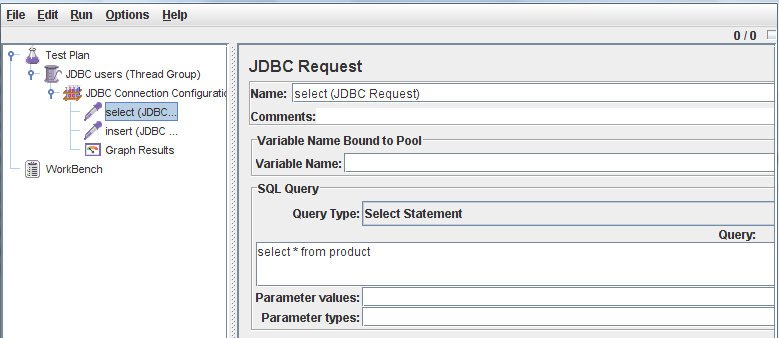
\includegraphics[width=13cm]{img/JMeterSQL.jpg}	
	\end{center}
	\caption{JMeter GUI}
	\label{JMeter}	
\end{figure}

Moreover these load tests can also be executed concurrently by JMeter and in two different ways:
\begin{itemize}
	\item Each thread group can simulate a collection of users with the same behavior. Each user is a thread, and the amount of thread is a parameter of the thread group. Therefore it's possible to simulate different users with the same behavior.
	\item It is also possible to implement different thread groups and so different behavior.
\end{itemize}
The ability to execute load test and concurrent test give us all the flexibility we need to run our test suite, particularly load test case such as the real time prepaid system explained at paragraph \ref{load-test-case}.

Another important feature in favor of JMeter is the capability to load test also databases via JDBC. As already said the figure \ref{JMeter} is an example of a JMeter configuration test for a database via JDBC. It shows how to simulate a group of user with the same behavior: they firstly execute a select and then an insert. The whole database configuration is setted up by the JDBC Connection Configuration where we need simply to specify the driver to be used and the usual connection parameters, such as the database URL, username and password. 

\begin{figure}[!htp] 
	\begin{center}
		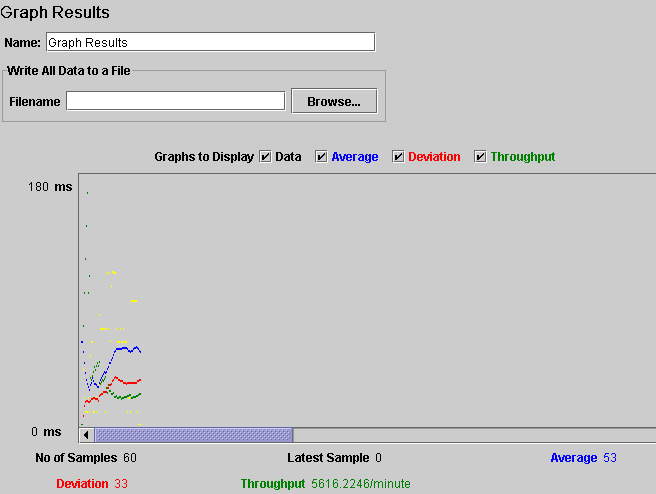
\includegraphics[width=13cm]{img/JMeterGraph.jpg}	
	\end{center}
	\caption{JMeter Graph}
	\label{JMeterGraph}	
\end{figure}

In figure \ref{JMeter} there is another element which we have not still explained: the Graph Result. JMeter is also capable to represent the results in a graphical form. In figure \ref{JMeterGraph} there is an example of a very simple graph obtained during a database load test (this image is taken from the Apache JMeter tutorial). This Graph Result is only a specific Listener which is possible to configure in the test plan, but there are many other listeners such as Table Result or Monitor Result and so on. It is also possible to execute JMeter from the command line interface, saving precious resources while running the test, logging all the results in a file, and then use a specific application to represent them in better ways.

Last but not least, JMeter is based on a plugin architecture and therefore it is highly extensible. Every element can be extended. For example a new Listener with a particular graph can be added, and also new Timers. This feature makes JMeter really flexible, and so another requirement is accomplished.

		\subsection{Disadvantages}
To make this analysis complete, we have also to evaluate the disadvantages of JMeter. And, as first thing, it's evident how JMeter doens't allow load testing of in-memory databases or other kind of databases which don't have a JDBC interface. It only acts with databases through SQL, and it is quite obvious: at the moment there is no a standard for database native interface. Therefore, although JMeter works with relational databases, it will not work with all the in-memory databases without a proper extension, an implementation of a new plugin, because there is no plugin available for our needs.

Moreover JMeter doesn't compare different systems between them, but instead it measures the performance of one system at time. Therefore there is no direct comparison, while the comparison is our main purpose. In fact JMeter was originally designed to test web applications in order to find the best tuning for the web server and the relative application. This means that JMeter is not used to find the best web server with the same application, which in other words it can be said that it is not used to find the best database for our application scenario. Nonetheless it can be also used to compare different systems, but not with much ease of use.

Also the visual representation of the result, the Graph Result, is not that great, and of course JMeter is not famous for graph results. It is not very fluid, and it has some bugs, such as when the test time is too much the graph goes in overflow.

		\subsection{Conclusion}
Now, after the analysis of advantages and disadvantages, we can conclude this investigation about Apache JMeter. It seems a very interesting application benchmark with a lot of features which meet most of our requirements such as:
\begin{itemize}
	\item portability, because it is written in Java and it is a desktop application;
	\item flexibility, which comes from the plugin architecture;
	\item ease of use, tanks to the GUI;
	\item visual and detailed report.
\end{itemize}

Although all these advantages, there is still something which is not perfect. Firstly JMeter can't test both object and relational databases, and this is an important limitation considering our main purpose is to test in-memory databases. Nonetheless JMeter can test java objects, and therefore it can work with java native interface, and however it is possible to write a new plugin to add the functionalities we need. But this solution will also add a considerable amount of work in programming the new plugin, losing partially or completely the usefulness of an already existing application benchmark.

Secondly also the graph listeners already implemented in the application are not very useful. They can only be used for a fast and approximate analysis. In order to create a good graph with the resulting data stored in a file, there are two possibilities: implement a new graph listener or use another application to represent the result. In both cases there is again the necessity to write new code's lines.

In addition JMeter doesn't allow an easy comparison between different results, and therefore, with the purpose to compare several database performance, there is no more ease of use.

Finally, JMeter is a great application and the extension with new plugins and other elements is very attractive, especially considering this is an open source application widely used. But not only the amount of code to write may be equal or more than the code needed to write a specific application for our needs; in this way we are also forced to move in a more complex application, although JMeter is easily extensible. However, taking in mind JMeter is not the best application to compare different performance, this is not a proper way to work. Nevertheless the extension of JMeter is still very interesting.
	
	\section{Poleposition} \label{poleposition}
Poleposition is an open source database benchmark, developed to compare database engines and object-relational mapping technology. Poleposition is built to be a framework to help developers in evaluating databases performance, through a simple implementation with only few lines of code. In fact the impetus behind Poleposition came from the observation that developers evaluating candidate databases for future applications often resorted to constructing ad hoc benchmarks rather than using "canned" benchmark tests (or relying on vendor-provided data). This is entirely understandable: to properly evaluate a database for a specific project, you would want to exercise that database in ways that correspond to the application's use of it \cite{poleposition}. This is the same concept we have already explained in paragraph \ref{categories} and paragraph \ref{axiom}.

Poleposition use the metaphor of a race, how it is clear by its name, to help the developers in understanding the framework structure.

		\subsection{Advantages}
This is another really interesting database benchmark, full of advantages. Above all, again, it is a Java desktop application, without the need of any installation, except for eventual database servers. Therefore the portability specified as first of our requirements is granted, allowing the test of database systems on different platforms.

In addition also the flexibility is provided by Poleposition: in fact it is a framework, for database benchmarking, allowing the implementation of new tests and of new database systems. The framework is also simplified by the metaphor used to describe the whole application,and which is evident by the name itself. This application benchmark is configured like a championship car racing, where:
\begin{itemize}
	\item A \emph{circuit} is a set of timed test cases that work against the same data.
	\item A \emph{lap} is a single (timed) test.
	\item A \emph{team} is a specific database category or engine that requires specific source code.
	\item A \emph{car} is a specialized implementation of a team, and therefore every database system can use several implementations.
	\item A \emph{driver} is an implementation of a circuit for a team .
\end{itemize}

In favor of Poleposition there is also the reporting tool: results are available both in HTML format and in a PDF file, providing a fast and clear idea of the results obtained. The PDF file and the HTML result are a collection of circuits, which actually are:
\begin{itemize}
	\item Melbourne: writes, reads and deletes unstructured flat objects of one kind in bulk mode.
	\item Sepang: writes, reads and then deletes an object tree.
	\item Bahrain: write, query, update and delete simple flat objects individually
	\item Imola: retrieves objects by native id.
	\item Barcelona: writes, reads, queries and deletes objects with a 5 level inheritance structure.
\end{itemize}
These circuits are a collection of laps: a write, a read, a delete etc. And each lap show the numeric results with both a table (table \ref{poleposition-table}) and a graph (figure \ref{poleposition-time-graph}).

\begin{table}[htp!]
	\centering \footnotesize
	\begin{tabular}{| r || c | c | c | c |} \hline
	t [time in ms] & objects:3000 & objects:10000 & objects:30000 & objects:100000 \\ \hline \hline
	db4o/6.4.14.8058 &	379 & 7365 & 1398 & 4820 \\ \hline
	Hibernate/hsqldb & 716 & 799 & 2617 &	14916 \\ \hline
	Hibernate/mysql & 1442 & 2948 & 9437 & 35853 \\ \hline
	JDBC/MySQL & 2881 & 1872 & 5470 & 18422 \\ \hline
	JDBC/Mckoi & 1202 & 2842 & 9371 & 33530 \\ \hline
	JDBC/JavaDB & 970 & 907 & 5454 & 8676 \\ \hline
	JDBC/HSQLDB & 276 & 57 & 199 & 931 \\ \hline
	JDBC/SQLite & 20381 & 46545 & 138990 & 483594 \\ \hline
	\end{tabular}
	\caption{Poleposition time table: melborune circuit and write lap}
	\label{poleposition-table}
\end{table}

The table \ref{poleposition-table} shows the time the "write" lap takes during the melbourne circuit. For each car/team is shown the time in milliseconds they take to execute a certain number of writes: 3000, 10000, 30000 and 100000. Therefore it's easy to compare them and understand who is the fastest, the winner of the race. The same result is also represented by a graph, figure \ref{poleposition-time-graph}, which clearly shows which database is above the others. To note how on the y axis the time is in a logarithmic scale and therefore higher is the value and faster is the database system. On the HTML result there is also another kind of chart, which measures the memory consumption, but on the PDF file this is not present.

\begin{figure}[htp!] 
	\begin{center}
		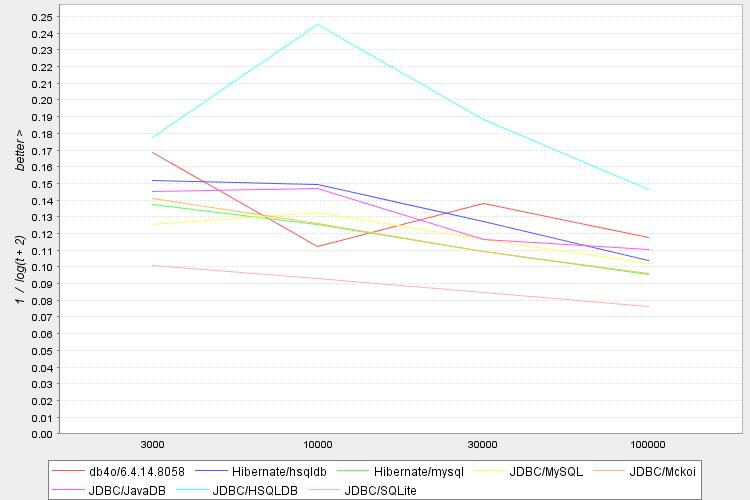
\includegraphics[width=13cm]{img/melbourne-write-time.jpg}	
	\end{center}
	\caption{Poleposition time graph: melborune circuit and write lap}
	\label{poleposition-time-graph}	
\end{figure}

Poleposition can also be used to test both object and relational database systems. This is possible because it was developed with the aim to compare database engines and object-relational mapping technology. Hence this makes poleposition a really interesting database benchmark for our needs.

Finally, as last advantage, there is something that is not properly a feature of the application, instead it is an idea the programmers took in mind during the development of the application, and therefore it reflected on the quality of the application. The idea we are talking about is the following:
\emph{"Objectivity must be the most important goal of the benchmark tests. The results show very clearly that there can not be one single best product. Depending on your application, some circuit results may be very important for you and some may be completely irrelevant."} 
This statement perfectly accords to the axiom described in paragraph \ref{axiom}, and on which is based our work.

		\subsection{Disadvantages}
The metaphor may help to understand the initial problem of the benchmark, but on the other hand, it becomes a trap, a limit for the benchmark itself: if they continue with the car race they will soon run out of gas \cite{poleposition}. Any further extension will be forced to follow the rail imposed by the metaphor. Moreover this metaphor makes the benchmark a simple race, and there is no load testing.

Although poleposition's output is very catchy, it is not easily readable and it lacks of detail: time and memory are the only measures taken in the HTML result and in the PDF file only the time is represented. In addition every test and graph/table lack of an explanation of what it is testing and representing, making the comprehension both of the test and the result very opaque. 

Moreover the results are always too much summarizing. For example in figure \ref{poleposition-time-graph}, and thus also in table \ref{poleposition-table}, only the total time of the test is represented, and so we can calculate the throughput dividing the number of objects inserted with the total time. But it's not possible to know if this throughput was constant or growing or oscillating too, there is no representation of the throughput's trend during the execution of the test. This contributes to make the test even less clear, hiding the real database systems' behavior. For example, looking at figure \ref{poleposition-time-graph}, we can't understand why HSQLDB and Db4o are so much oscillating. Of course it can be the real database performance, but it could also be a mistake in the test implementation or in the database configuration. Certainly a more detailed report of the result could be helpful.

Furthermore this framework only allow single-user testing, because, as the authors said in \cite{poleposition}, \emph{"some sort of multi-threaded test to simulate multiple user would be exceedingly difficult without extensive modifications to the framework. But if that could be done, PolePosition could provide enterprise-level testing"}. Nevertheless they hope in the future to introduce this new functionality, but at the moment it is still not working.

Finally this database benchmark is quite recent: it started in 2005 and actually there is still only one release available for download, posted in June 2005. Looking through the SVN repository on sourceforge, it's possible to notice some new changes and activity in the last years, but there is still no new release available for download. In addition the code of poleposition is not that clear and object oriented as they said in \cite{poleposition}.

%oltretutto compara e basta ma non misura performance
		\subsection{Conclusion}
As first impact Poleposition seems to be exactly what we are looking for:
\begin{itemize}
	\item the portability is granted by the Java language;
	\item new test can be implemented allowing flexibility;
	\item there are very catchy graph report;
	\item and it can works both with relational and object databases.
\end{itemize}
But a deep analysis of this feature showed that it is not suited for our needs. Particularly the results are very poor, and the graphs don't show any database behavior during the execution of the test: in fact these graphs shouldn't be line charts, but it would be better if they were bar charts, because they don't show any trend.

But a very important disadvantage, which exclude Poleposition from our choice, is the lack of load testing, also due to the incapability to execute concurrent tests. This is a major disadvantages, especially when we want to simulate real application scenarios, which is a consequence of the axiom on which is based our work. 

In addition this benchmark is not easy to use, although it may seem easy. It's impossible to understand the meaning of the results without looking at the code: \emph{"if you consider basing your choice of database on this benchmark, bring along lots of time to look at what every test does. You will not be able to judge the results without looking at the source code that produces them."} And therefore this benchmark is not for non technical people who don't know Java language, but also for engineers is not so easy, because they need a lot of time to understand properly the benchmark results, looking through the code's lines.

It could be possible to extend this framework with the features we need and the authors themselves exhort this possibility. On top of that there is a substantial amount of code to write and the framework code is not simple and easily extensible: for example there are methods with hundreds of line of code and with many many nested conditional instructions, which is not object oriented programming, losing all the maintainability such a programming paradigm offers.

However this application is very catchy and it is a great source of inspiration for a future development. Very interesting features, although they are not perfect, are the report in a PDF file, the graphs, and the idea to make a database benchmark framework.
	
	\section{Benchmark Overview Summary}
Coming to a conclusion we sum up the pros and cons of the database benchmark applications analyzed in the table \ref{benchmark-summarizing-table}. It shows only the most interesting negative and positive features we found in these benchmarks, in order to understand what we need and take inspiration for a future development of a new benchmark application.

\begin{table}[htp!]
	\centering \footnotesize
	\begin{tabular}{| p{2.5cm} || p{5cm} | p{5cm} |} \hline
	
	Benchmark & Pro & Con \\ \hline \hline
	
	\multirow{5}{2.5cm}{The open source database benchmark} &  & SQL only \\
	& Open source & C language \\
	& AS3AP & No comparison \\
	&  & No visual reports \\
	&  & Latest release: 0.21 (2006) \\
	\hline
	
	\multirow{5}{2.5cm}{TPC-C benchmark} & Standard &  \\
	& Simulate OLTP systems & For high end vendor \\
	& Price/performance metric & No implementation available \\
	& Acidity testing &  \\
	& For every DBMS &  \\
	\hline
	
	\multirow{4}{2.5cm}{Apache JMeter} & Java desktop application & No plug-in for IMDB \\
	& Load testing & No comparison \\
	& Plug-in architecture & Bad graphs \\
	& JDBC plug-in &  \\
	\hline
	
	\multirow{5}{2.5cm}{Poleposition} & Java desktop application & The metaphor is a trap \\
	& Database benchmark framework & Lack of detail in results \\
	& Both relational and object DB & Only single-user testing \\
	& Results comparison & Quite recent \\
	& Catchy report &  \\
	\hline
		
	\end{tabular}
	\caption{Benchmark summarizing table}
	\label{benchmark-summarizing-table}
\end{table}

The starting idea was to find an application with the requirements explained in paragraph \ref{requirements}, so that we could be able to run our test suite. But the final result is that there is no benchmark which perfectly fits our needs. This means there are only two possibilities to execute our test suite:
\begin{itemize}
	\item choose one of the benchmarks previously analyzed and then extend it, in order to add the functionalities we are looking for;
	\item develop a new benchmark starting from our requirements.
\end{itemize}

The first idea was already taken into consideration during the benchmark analysis and rejected in the conclusion paragraphs. In summary:
\begin{itemize}
	\item The first benchmark, the open source database benchmark, was completely unsuitable. Not even one requirement was satisfied. The only positive aspect was the use of AS3AP, the ansi SQL standard scalable and portable benchmark (portable only for relational database server), which can be helpful to the creation of new test case.
	\item The transaction processing performance council, with their TPC-C, is very interesting because it is a standard and it can simulate a generic OLTP system. But there is no implementation available, and anyhow this will not help us to execute are test suite. Instead this can be a good source for inspiration, both for a new load test case and for some ACID test case. So it is a nonsense talking about extension.
	\item Apache JMeter is a very good general purpose benchmark application and offers a plug-in for testing relational database server through JDBC. Therefore to use this tool for our aim we need to write a new plug-in, which may not worth the effort, especially considering that JMeter allows an efficient measurement of the performance, but not an easy comparison between different system, and moreover the graphs are quite poor, although extensible.
	\item Poleposition, on the other hand, is suited for both relational and object database systems, but its testing capability are quite poor. The lack of concurrent testing, and therefore of load testing, prevent us to execute our test suite. A possible extension of this application is not the best solution, especially looking at the source code which is not well organized.
\end{itemize}

Therefore the best solution is to develop a new benchmark application. Although this decision, the analysis done is not useless, in fact we understood which features can be used from other benchmarks, and how to develop them, and what should be avoided. But this will be explored in the next chapter.
	
\chapter{The New Database Benchmark Application}
The previous chapter is dedicated to the research of a suitable benchmark application for our needs which is able to execute our test suite. The analysis didn't bring to any available benchmark neither to a benchmark easily extensible in order to implement the features we want. Therefore the conclusion was to develop a new benchmark application, starting from our requirements and treasuring the knowledge acquired during the analysis.

In this chapter we describe the new benchmark application developed for our needs, starting form the specification defined from the requirements and then describing the application from different points of view. Subsequently we will discuss also about the application usage, from the application's configuration to the extension and the implementation of new databases and tests.

	\section{Analysis: Requirements Specification}	
	%Then the focus is moved on the design, describing and representing the application by different point of view: functional, information, concurrency and development.
	
This section is dedicated to the analysis of the benchmark application developed during this thesis. We start from the specifications' definition, which come from the requirements described in paragraph \ref{requirements} and from the functional requirements resulting from the capability to execute the test suite described in chapter \ref{test-suite}.
	
In order to define the specifications from the requirements on which the benchmark application is based, it's primarly important to understand what is a specification in relation to requirements. A requirement is a singular documented need of what a particular product or service should be or do. On the other hand a specification is an explicit set of requirements, or in other words it is a well-formed requirement, a formal requirement, an implementable requirement. 

Now it is clear how the discussion done in chapter \ref{overview} is not useless. Through that analysis we obtained a better understanding of the requirements, and a suggestion to implement them. This will help us in the process of requirements specification. 

The table \ref{benchmark-specifications-table} summarizes the specifications we are going to analyze in the following paragraphs. 

\begin{table}[htp!]
	\centering
	\begin{tabular}{| p{6cm} | p{6cm} |} \hline
	
	\bfseries{Requirements} & \bfseries{Specifications} \\ \hline \hline
	
	Portability & Java \\ 
	\hline
	
	Understandability & clear PDF file with graphs \\
	\hline
	
	Flexibility & extensible framework  \\
	\hline
	
	Detailed Report & several measures \\
	\hline
	
	Visual Report & graphs with trend \\
	\hline
		
	Both Relational and Object Databases & databases interface written in Java \\
	\hline
	
	Ease of Use & XML both for test and report configuration\\
	\hline		
	
	\end{tabular}
	\caption{Benchmark specifications}
	\label{benchmark-specifications-table}
\end{table}


		\subsection{Portability}
We already recognized the value of portability as a requirement when testing embedded databases, because it allows us also to chose the best platform for the database we are testing and to study the difference in the performance with a platform's change. From the experience gained with the benchmarks' analysis we know that both JMeter and Poleposition grant the portability we need. And this is granted thanks to the Java language. In fact they are both Java desktop application who are able to be executed on several platform because the Java Virtual Machine allows Java to run everywhere (\emph{"write once, run everywhere"}).

Therefore this requirement brings to a simple specification: when you want to grant portability to an application, the Java language is a good solution. 
		
		\subsection{Understandability}
When a benchmark is not easily understandable, it is useless. Benchmarks are too easily tricked and cheated, and thus they are meant for different stakeholders. Looking at JMeter and Poleposition we understand how a graph can help to explain the numeric results and to compare several systems. Particularly Poleposition offers a very catchy PDF result, containing all the tests with all the results expressed both in tabular and graphic results. But in this PDF what the test does is not very clear. Then the need of clear results which explain also the test's operations. For this purpose JMeter is a bit better, because with a tree structure it shows exactly the task and all the operation involved by the test.

Therefore what we need to grant this requirement is a PDF result, containing all the information about the tests: 
\begin{itemize}
	\item what the test does, in terms of operations involved on the database;
	\item graph result which catch the attention of the reader and quickly express the meaning of the numeric result.
\end{itemize}
This is the specification implicated by understandability.
			 
		\subsection{Flexibility}
Benchmark always suffers the limitation introduced by the workload simulated. The performances measured by the benchmark are highly dependant on the workload, and therefore for an application, whose workload is not similar to the benchmark's one, the results are nearly useless. To overcome this limitation, flexibility is a key feature. In this contest flexibility is meant as the capability of the benchmark application to run complete new tests, and so to simulate new workloads. Furthermore it is also intended as the capability to run the benchmark against new database systems. Also this time JMeter and Poleposition show a possible solution to this problem, but they are not equals.

As regards Poleposition, it works like a framework, in fact the main idea behind this application is to make a framework for databases benchmarking. Therefore Poleposition allow an easy implementation for both new tests and database systems, although it is not so easy and flexible as a framework should be, especially for new tests. In both cases the solution involves the programming of new code's lines.

JMeter, instead, is able to create and execute new tests thanks to a graphic editor which can be used to create very complex scenarios. In regard to the implementation of new database systems, at the moment JMeter can test only SQL databases, but a possible solution may be the development of a new plug-in. In fact JMeter is based on a plug-in architecture, which allow a good evolution of the software.

In conclusion the resultant specification is: create a benchmark application which works as a benchmark, with tests that can be implemented by programming, and with pluggable databases.
			 
		\subsection{Detailed Report} 
A well detailed report with a lot of interesting measures will tell you much about the databse behavior, while only one single metric will simply make your trust go away when you read it. 

The first who stated this idea was the transaction processing performance council, who, in fact, adopt two different measures: the first is the throughput and the second is a price/throughput measure. This beacuse the TPC-C benchmark doen't compare directly different systems, but every vendor run it on his own, therefore without a price/performance measure, it is very hard to understand if the result depends from more expensive computers. This is not our case, but we agree that one measure doesn't exaplain the real database performance.

JMeter, instead, has several listeners which are able to take different measures, and they can be composed in many ways inside a test plan. So JMeter allows the user to take exactly the measures he wants. And this is applicable also for graph listners.

In this case case JMeter shows a very good solution, and this is exactly what we like: the possibility for the user to chose the measures to display as final result.
			
		\subsection{Visual Report}
When you face complex results with a lot of numbers, a visual representation will make them clearer. Thus when using graphs also a comparison between different systems will be easier, because it becomes a comparison between different colored lines. Furthermore graphs are very helpful if you want to analyze not only the final result of a test, but the whole trend.

Although Poleposition makes use of graphs, these don't represent any test's trend, they simply represent the final value of the test. Nevertheless Poleposition with its graphs allow a very easy comparison between different database systems and the graphs are very catchy.

On the other hand JMeter provides very stark graphs, without any comparison between different systems. But it is possible to represent each measure on the graphs and in addition they show the performance's trend during the test's execution. Using appropriate listeners, or writing new ones, it is possible to represent almost everything.

To sum up we want graphs who let us compare different database systems and draw different measures, with the capability to analyze the trend during the test's execution, but in a catchy way. Something like Poleposition graphs with in addition the trend representation. Furthermore the user should chose which graphs create, specifying the measure to drawn on the graph's axis.
			 
		\subsection{Both for Relational and Object Databases}
Relational and object database system usually doesn't share the same interface. From the Java point of view, relational databases are usually accessed through JDBC, while object databases usually use native interfaces. It's not easy to make a database benchmark work with two different technologies, there is an impedance mismatch. 

Poleposition is able to test both relational and object databases, but at the cost of a completely new implementation of the whole test for every database which is to be tested. JMeter instead works only with relational databases, but it provides also the possibility to test Java objects, which is very useful thinking at Java native interfaces to access the databases. Nevertheless this means that an object oriented point of view will be used for object databases and at the same time a relational point of view will be used for relational databases, therefore the final result will have less meaning. With the purpose of benchmarking and comparing it's better to use a uniform point of view.

Since the benchmark application we want to develop must work with both relational and object database systems and since most of our database are object databases, we will use an object oriented point of view when benchmarking databses and therefore every database must implement a Java native interface for each test. Every database must implement a own interface, a driver, because there isn't yet any standard for object oriented querying.
			 
		\subsection{Ease of use}
Easy of use is intented as a variation in the tests'parameters, such as the initial database state and others already explained in chapeter \ref{test-suite}, allowing little variations to the workload simulated, in order to improve the test when the needs change. 

This ease of use should be granted without any modification in the application's lines of code. For this purpose Poleposition uses several properties files while with JMeter the user can modify the whole test, without any programming, and therefore he can also modify every parameters in the test without touching any code's lines.

Our idea consists in an xml file which contains all the tests' configuration. The xml file should be organized with a tree structure such as the JMeter's representation of the test plan. This xml must contain all these variable parameters. Furthermore we would like to configure also the final report of the benchmark, specifying which graphs draw and which measures represents for each test.

		\subsection{Test Suite's Specification} \label{test-suite-specification}
More specifications come from the capability for the benchmark application to execute the test suite described in chapter \ref{test-suite}. These are functional specifications because they describe the requested application's behavior. In this particular case, therefore, they come from the test suite and we are going to analyze them. 

In order to run the test suite we need the benchmark to be able to:
\begin{itemize}
	\item execute test concurrently and therefore allocate a thread for each task composing a test; 
	\item run each task of the test at most for a specific amount of time, which may be different for every task;
	\item iterate each task for a certain maximum number of iteration, different for each task;
	\item run each task without consuming all the resources and therefore limiting the transactions per second, the throughput of the task.
\end{itemize}
All these informations must be taken by the benchmark application as input without any programming, and therefore they must be specified in the XML file.	
		
		
		
	
	\section{Design And Development}
Software design is a process of problem-solving and planning for a software solution. After the purpose and specifications of software are determined, software developers will design or employ designers to develop a plan for a solution. It includes low-level component and algorithm implementation issues as well as the architectural view.

In this section we will design and develop the application using different point of view, or it's better to say we will show how the system has been realized by describing it through different point of view. Although a common temptation is to try to analyze and describe a system with a single, heavily overloaded model \emph{"it's not possible to capture the functional features and quality properties of a complex system in a single comprehensible model that is understandable by and of value to all stakeholders"} \cite{SSA}.

Therefore different views will be used in the following paragraphs to describe separatly each the major aspect of the benchmark application. The views used are the functional view, the information view, the concurrency view and the development view. Collectively they describe the whole system. 

		\subsection{Functional View}
A functional view defines the system's functionalities, demostrating how the system performs the functions required. This is probably the easiest view for stakeholders to understand the system and it is the starting point for the definition of the other architectural views. The figure \ref{system-external-view} represents the benchmark application from a functional point of view which takes into account the specifications summarized in table \ref{benchmark-specifications-table}. It represents the system by an external point of view, showing functional capabilites, external interfaces, internal structure and design philosophy, such as the low coupling between the database and test implementations.
		
\begin{figure}[htp!] 
	\begin{center}
		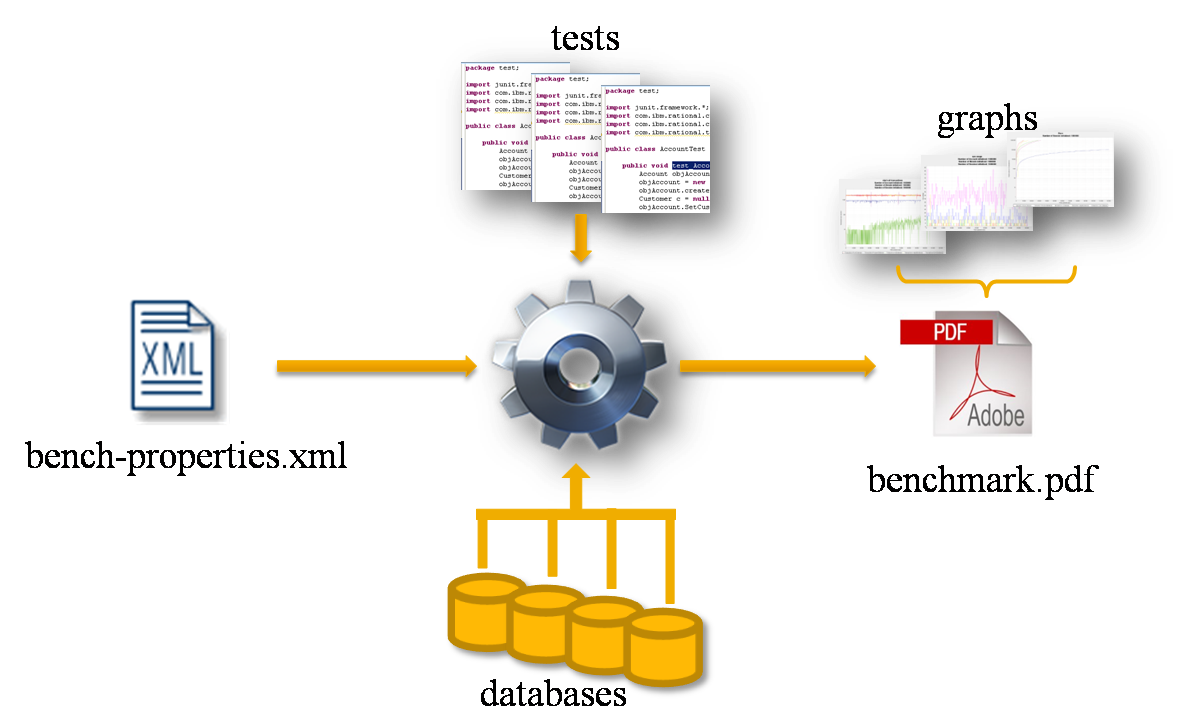
\includegraphics[width=13cm]{img/diagramma-specifiche.png}	
	\end{center}
	\caption{Functional view: the system from an external point of view}
	\label{system-external-view}	
\end{figure}

The benchmark application, represented in the figure \ref{system-external-view}, is composed with the following parts:
\begin{itemize}
	\item The application's input is an XML file, the bench-properties.xml. It contains a substantial part of the tests' configuration, that is a colletion of variable parameters for each test, such as the task, the operations' order, the time, the maximum throughput, the initial database's state etc.
	\item The group of databases shows how they can be plugged in the benchmark, in order to execute benchmark's tests on several and new databases.
	\item New tests can be implemented in the benchmark application allowing the execution of specific workloads. 
	\item The output is a PDF file cointaining all the results obtained by the performance analysis.
	\item The results in the output file are represented mostly by graphs.
	\item Finally a gear represents the application as a black box. The figure just shows that the application works as a framework with extensible databases and tests.
\end{itemize}
In other words, the benchmark application takes as input an XML file, and through pluggable databases and tests, it produces a PDF file containing all the result, represented also with graphs.

		\subsection{Information View}
The information view focus on a small number of entities that your stakeholders view as significant or meaningful, primarly considering the user stakeholders, but also taking into account the concerns of other stakeholders types such as maintainers. The idea behind the model is to keep it simple. Although our application doesn't store any information, it manipulates, manages and creates information.

The figure \ref{information-view} can be considered a kind of information view because it describes the entities involved by the benchmark application. Anyway this model is very useful because it provides a description of the entities, helping the comprehension of how the benchmark works. This view is not only for developers who can eventually implement new features and extend the current application, but it is dedicated to every stakeholders. In fact it explain very well how a test works and how it is composed, and this comprehension is essential for a right use of the XML file, but is is even essential for understanding the benchmark's results.

\begin{figure}[htp!] 
	\begin{center}
		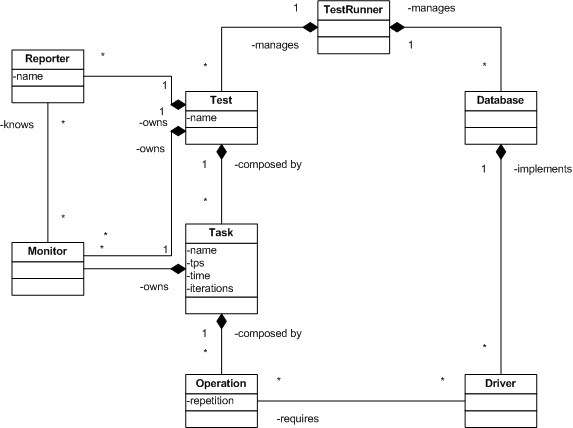
\includegraphics[width=13cm]{img/uml.jpg}	
	\end{center}
	\caption{Information view: class diagram}
	\label{information-view}	
\end{figure}

Analyzing more in detail the figure \ref{information-view}, it is so composed:
\begin{description}
	\item[Test]: this is the most important entity in the benchmark application. It represent the test which can be started on a specific database. Each test has a name which is configurable by the XML and helps the readability of the output. Furthermore each test is composed by tasks and has a collection of monitors, which measure the test's performances, and reporters. 
	\item[Task]: this is substanatially a set of operations which are executed synchronized. Each task has also a collection of monitors which measure the task's performances. As for the test, also the task got a name to help the readability of the PDF file, but, very interesting, are some special attributes which are used to define the test scenario to simulate. These attributes, setted in the XML file, are the transactions per second (tps), the time and the number of iterations. They have been already explained as specifications in paragraph \ref{test-suite-specification}.
	\item[Operation]: this is the class to write to extend the database benchmark framework. Every operation represent one or more method invocation to the database. 
	\item[Monitor]: this entity is dedicated to the performances' measurement. It monitors some specific measure of the test/task to which it is linked, such as the throughput or the cpu usage.
	\item[Reporter]: this is a monitor of monitors. In fact they register and put togheter several measures of different monitors. This entity is dedicated to the production of graphs in the output file, and therefore it also has a name, helping the readability. A reporter can be declared directly in the XML file and can represent exactly what the user wants.
	\item[Database]: this entity represents a specific database, such as Prevayler, Pico4 or HSQLDB. It is a collection of drivers.
	\item[Driver]: this is a driver required for the execution of a specific operation, which may require also more than one driver. In other words this can be seen as the implementation of a specifica database for an operation.
	\item[TestRunner]: this entity runs the benchmark, executing every tests on every databases. In fact it manages a collection of test and another collection of databases.
\end{description}

		\subsection{Concurrency View}
The concurrency view describes the concurrency structure of the system, mapping functional elements to concurrency units to clearly identify the parts of the system that can execute concurrently, and shows how this is coordinated and controlled.

The concurrency of our benchmark application is very simple, and it is based only on threads, but an exaplanation of it will help in the comprehension of how tests work and, therefore from the definition of new tests and databases to a "consapevole" results' analysis. 

\begin{figure}[htp!] 
	\begin{center}
		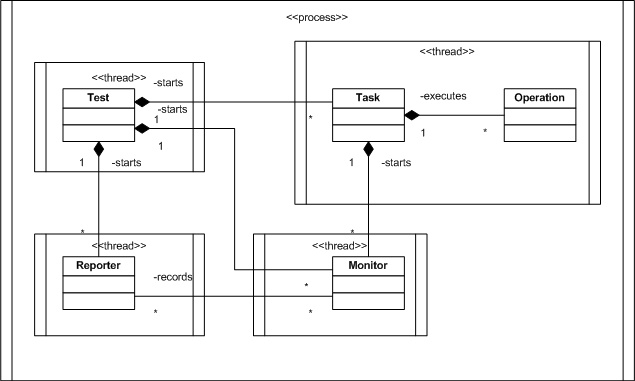
\includegraphics[width=13cm]{img/concorrenza.jpg}	
	\end{center}
	\caption{Concurrency view: threads}
	\label{concurrency-view}	
\end{figure}

The figure \ref{concurrency-view} shows how the concurrency is organized, mapping the active entities, already seen in figure \ref{information-view} in the previous paragraph, to threads. The benchmark runs in only one process of the operating system, in the Java virtual machine, except the processes of the in-memory databases. All the other concurrent elements are divided into different threads:
\begin{itemize}
	\item The is only one test running per time, and after it starts the reporters, the monitors and the tasks it waits the end of every tasks.
	\item Each monitor is associated with a thread so that they can measure the performance of the test and of the different task concurrently.
	\item Each reporter runs in a own thread, and, after it is started by the test, it records the values measured by the monitors.
	\item Each task is executed concurrently with the other tasks and so there is a dedicated thread for each task. After it starts the monitors associated, it executes in a repetitive and synchronized way all the operations which compose the task itself.	Therefore all the operations belonging to a specific task are executed in the same thread.
\end{itemize}

		\subsection{Development View}
A considerable amount of planning and design of the development environment is often required to support the design and build of software for complex systems. Things to think about include code structure and dependencies, build and configuration management of deliverables, system-wide design constraints, and system-wide standards to ensure technical integrity. It is the role of the development view to address these aspects of the system development process. The concerns of the development view we will analyze are the modules organization, the codeline organization and some of the technologies used by the application. Furthermore we will also analyze an UML sequence diagram for a test's execution.

			\subsubsection{Module Organization}

As regards the module organization, the figure \ref{development-view}, which is simply a screenshot of the project inside the Eclipse IDE, describes the package organization. There are three main packages in which the whole application is divided:
\begin{itemize}
	\item The test package contains the tests with all their operations which is possible to execute and configure in the XML file.
	\item The database package contains, for each database system, the implementations for the tests: the drivers which are required by the operations, enabling them to operate, hiding the specific database implementation. In fact, these drivers are adapters for the database systems' diversity.
	\item The core package is the hearth of the benchmark application and contains all the framework: from the monitors to the reporters and to everything is needed to execute the tests on the databases.
\end{itemize}
In fact our application is built as a framework for database benchmarking, ensuring the extension with new tests and databases implementation. Therefore both tests and database have a dedicated package, in which they can be written and plugged-in without the necessity to know the whole application. Furthermore these three packages have few dependencies which in addition are managed only through indirections, such as interfaces and adapters.

\begin{figure}[htp!] 
	\begin{center}
		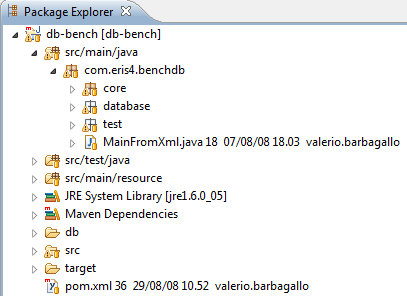
\includegraphics[width=13cm]{img/development-view.jpg}	
	\end{center}
	\caption{Development view: Eclipse's package explorer}
	\label{development-view}	
\end{figure}

			\subsubsection{Codeline Organization}

As regards the codeline organization, the system's source code needs to be stored in a directory structure, managed via some form of configuration management system, built and tested regularly, and released as tested binaries for further testing and use. The way that all of this is achieved is normally called the codeline organization. The figure \ref{information-view} not only shows the division in package of the source code, but it shows also the whole project structure, the codeline organization. Eclipse's users probabily have already recognized Maven, a software project management tool which is integrated in Eclipse with thanks to a plug-in. Maven simplifies the build project, provides a uniform build system on different platforms and has a superior dependency management, and it is managed with the pom.xml file, where all the settings are placed, such as the dependencies. 

Eclipse's users will also notice the small database symbol which means that the project is hosted on a repository. In particular the application is on a SVN repository: the exact URL for the repository, which is available for everyone in internet, is at \lstinline[commentstyle=\color{black}]!http://portable-db-bench.googlecode.com/svn/trunk/!, which is a free SVN repository offered by Google. In fact our project is open source and any contribution is welcome.

			\subsubsection{Other Technologies}

As already exaplained, Maven manages the depending libraries in a very simple way. The question is now which dependecies we are using. Except all the dependecies involved by the database systems, there are three major technologies used by our application: log4j, jfreechart and itext.

Log4j is a very common library used by most programmers and it enables a uniform logging system for the whole application. This is low-tech method for debugging which is very useful with concurrent applications. The major advantage of log4j is the possibility to enable logginat runtime, without modifying the application binary using, moreover, different log levels.

Instead, jfreechart is used to create the graphs in the resulting PDF file. It is a free 100\% Java library which allows the creation of professional quality charts. A nice feature is the support for many output types, but there is also a great variety of available charts such as bar charts and pie charts, but the chart used by the benchmark application is an \lstinline!XYLineChart!: a 2D chart with x and y axis. It is suited to analyze the trend in the performance during the benchmark's execution.

Finally, also iText is noteworthy. It is a a free Java library that allows the creation of PDF files on the fly. It is build in the benchmark application, producing the PDF file containing all the results, generating a read-only, platform indipendent documents, containing also all the graphs/images produced by jfreechart.
			
			\subsubsection{Test's Execution}

In conclusion for the development view, we illustrate the sequence diagram for a test's execution, with the purpose to increase the comprehension of the life's cycle of a test. This will simplify both the use of the XML file taken as input and the implementation of new tests and databases. 

The figure \ref{sequence-diagram} is a UML sequence diagram and it shows a simplifyed test's execution, because it's not displayed the interaction with monitors and reporters. The focus is on the test, the task wich compose the test and the operations which compose the task, and their life's cycle.
		
\begin{figure}[htp!] 
	\begin{center}
		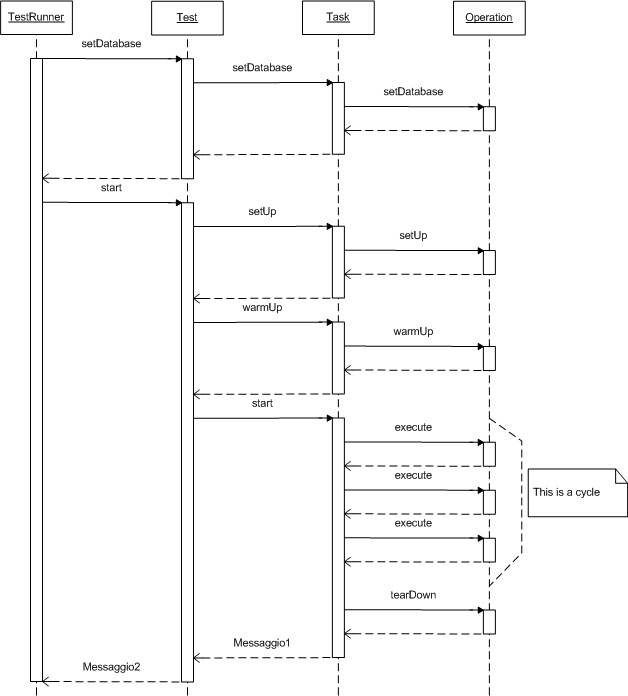
\includegraphics[width=13cm]{img/sequence-diagram.jpg}	
	\end{center}
	\caption{Sequence diagram for a test's execution}
	\label{sequence-diagram}	
\end{figure}

The sequence diagram how a test is executed and we can divide the execution in five phase:
\begin{enumerate}
	\item The \lstinline!TestRunner! is the main class who execute all the tests on all the databases, but before starting a test, a preliminary operation is done: the database is setted in the test so that the \lstinline!TestRunner! executes the test on a specific database. This operation spread to all components of a test, through the tasks to the operations, so that each operation can take the suitable driver from the specific database.
	\item In a second stage the test is started by the \lstinline!TestRunner!. Then the test sets up all its tasks and consequently all the operations. In other words this phase corresponds to an opening of the connection with the database.
	\item Subsequently the test warms up all its tasks and operations to avoid the slow start of the real test, when all performance measures are taken.
	\item In this stage the test starts a thread for each task, which then executes repeatedly, and concurrently with the other tasks, the operations.
	\item In a final stage, when the stop condition is reached, each task tears down the operations, which in other terms means a close, a disconnect from the database. The driver is detached.
\end{enumerate}
			
	\section{Application Usage}
While in the first section we analyzed the specifications on which the application is built and in the second the focus moved to the design, in this section we assume the application already developed and we analyze the application usage. The main use is of course the execution of the benchmark and therefore the configuration of the XML. But recalling that the application is structured as a framework, other kinds of use consist of the implementation of new tests and of new databases.

		\subsection{Configure the XML}
The benchmark application developed, as clearly showed in the functional view, takes in input an xml file: the bench-properties.xml. It contains the whole configuration for the benchmark's execution and it grants the ease of use so much researched. In fact it is possible to specify and change a lot of parameters such as the several stop conditions for the task, the test's composition, the reporters and more.

			\subsubsection{Training XML}
To take confidence with the XML, we start analyzing a training example, which can't be executed, but exaplains what every attribute or element is used for. This training XML is showed in the listing \ref{bench-properties-training}. It is divided into three parts.

The first part is full of definitions which are a mappings between a name and a class, so that we will not need to repeate all the path every time, but we can use a "key", which is a simple name. The definitions are divided into four parts: initializators, operations, test monitors and task monitors. We already know the operations and monitors, although they are classified differently for tests and tasks, but we don't know what is an initializator. It is a special class which is used to fill the database, in order to simulate scenarios where there is no empty database. For example, we can assume that our operations interact with the database writing and reading a certain object, a \lstinline!Person!. If we want to simulate a scenario where the database already contains one million of Person, we need a \lstinline!PersonInitializator!, a class which may be called by the Test before starting each task. Another clarification to mention is that if you declare a monitor as a task monitor, every task will use that kind of monitor, and on the other hand, if you declare it as a test monitor, every test will use it. Although you will probably never change the monitors' definition.

\begin{lstlisting}[language=xml,caption={Training bench-properties.xml},label={bench-properties-training}]
<bench>
	
	<!-- DEFINITIONS -->
  <definitions>
  	<!-- initializators -->
  	<initializator name="PersonInitializator" class="com.eris4.benchdb.test.person.initializator.PersonInitializator"/>
  	...    	
  	<!-- operations -->
  	<operation name="WritePersonOperation" class="com.eris4.benchdb.test.person.operation.WritePersonOperation"/>
  	...
  	<!-- test monitors -->
  	<testmonitor name="Memory" class="com.eris4.benchdb.core.monitor.MemoryMonitor"/>
  	...
  	<!-- task monitors -->
  	<taskmonitor name="Time" class="com.eris4.benchdb.core.monitor.TimeMonitor"/>
  	...    	
  </definitions>
	
	<!-- DATABASE LIST -->
	<databases>
		<database class="com.eris4.benchdb.database.pico4.Pico4Database"/>
		...
	</databases>
		
	<!-- TEST LIST -->
	<tests>
		<test name="Test 1" >
			<initializator name="Initializator 1" numberOfObjects="1000"/>
			<!-- More initializators here -->						
			<task name="Task 1" 
			iterations="The total number of transaction after the task stops" 
			time="The maximum time after the task stops" 
			tps="The maximum transaction per second">	
				<operation name="Operation 1" repetition="1"/>
				<!-- More operations here -->			
			</task>
			<!-- More tasks here -->
			<loggraphreporter name="Reporter 1">
				<line x="Time" xTask="Task 1" y="AvgTransaction" yTask="Task 1" name="AVG"/>
			</loggraphreporter>
			<lineargraphreporter name="Reporter 2">
				<line x="Time" y="Memory" name="Memory"/>		
			</lineargraphreporter>
			<!-- More reporters here -->
		</test>
	<!-- More tests here -->
	</tests>
</bench>
\end{lstlisting}

In the second part consists of a list of databases which will be tested. This is not a mapping like for the definitions, but it is simply a declaration of database, specifying the path of the class which extends the base class \lstinline!Database! of the framework.

The third part is the most important. In fact while the first and the second part are rarely modified, the third is used for the test configuration, containing all those variable parameters which often may be changed. In this part, every test element is a test which is executed on all the databases listed. Each test is composed by different elements:
\begin{description}
	\item[Initializator]: this element describes which initializators the test must execute to fill the database. There are two interesting attribute: the name is a pointer to one initializator defined in the first part with the same name, while the second attribute specifies the number of objects to insert in the database.
	\item[Task]: this is a collection of operations which are executed in a serialized way, and concurrently with the other tasks. While the attribute name is used only to create more clear results, the others are the key parameters of the test: 	
	
	\begin{itemize}
		\item The tps attribute is used to limit the throughput of each task. This is an optional attribute.
		\item The iterations attribute stands for the total amount of task's execution before the task is stopped. This is optional too.
		\item The time attribute is the maximum amount of time before the task is stopped. This is a required attribute and it is used also to avoid that a very slow database system can snooker the benchmark when only a the iteration attribute is used, therefore a sort of timeout. 
	\end{itemize}	
	
	\item[Operation]: this is an operation executed by the test inside a specific task. The name attribute is a pointer to an operation previously defined in the first part of the XML. The repetition attribute tells the number of time that an operation must be repeated for every task's execution.
	\item[Loggraphreporter]: this reporter uses a linear scale for the x axis and a logarithmic scale for the y axis.
	\item[Lineargraphreporter]: this reporter uses a linear scale both for the x and the y axes. 
	\item[Line]: this is used inside a reporter to specify what a reporter should draw. This element has several attributes:
	
	\begin{itemize}
		\item The name of the line.
		\item The x value to represent: this is a pointer to a monitor defined in the first part.
		\item The xTask which is a name used as a pointer to a task's name already declared in the current test, specifying to which task's monitor the x value is referred.
		\item The y value to represent: this is a pointer to a monitor defined in the first part.
		\item The yTask which is a name used as a pointer to a task's name already declared in the current test, specifying to which task's monitor the y value is referred.
	\end{itemize}
	
\end{description}

			\subsubsection{Real Time Prepaid System XML}

After a non executable example of the XML file, we now analyze a more complex and real XML file. It describes the main test case developed in our test suite which is described in paragraph \ref{real-time-test-case}. The listing \ref{real-time-prepaid-system-xml} shows only the main part of the xml file, the one containing the test's configuration, excluding the first and the second part, which are a simple list of definitions and databases. 

\begin{lstlisting}[language=xml,caption={Real time prepaid system XML},label={real-time-prepaid-system-xml}]
<test name="Telephone company use case">
	<initializator name="AccountInitializator" numberOfObjects="1000000"/>
	<initializator name="MsisdnInitializator" numberOfObjects="1000000"/>
	<initializator name="SessionInitializator" numberOfObjects="1000000"/>
	<task tps="10" time="120000" name="Balance check">
		<operation name="ReadMsisdnOperation" repetition="1"/>
		<operation name="ReadAccountOperation" repetition="1"/>						
	</task>	
	<task tps="10" time="120000" name="Account management"> 
		<operation name="WriteAccountOperation" repetition="1"/>
		<operation name="WriteMsisdnOperation" repetition="2"/>				
	</task>				
	<task tps="2000" time="120000" name="Service authorization and management">
		<operation name="ReadMsisdnOperation" repetition="1"/>
		<operation name="ReadAccountOperation" repetition="1"/>					
		<operation name="WriteSessionOperation" repetition="1"/>				
	</task>	
	<loggraphreporter name="Balance check transactions">
		<line x="Time" xTask="Balance check" y="Transaction" yTask="Balance check" name="Transactions"/>
	</loggraphreporter>
	<loggraphreporter name="Balance check AVG transactions">
		<line x="Time" xTask="Balance check" y="AvgTransaction" yTask="Balance check" name="AVG"/>						
	</loggraphreporter>
	<loggraphreporter name="account management transactions">
		<line x="Time" xTask="Account management" y="Transaction" yTask="Account management" name="Transactions"/>
	</loggraphreporter>
	<loggraphreporter name="account management AVG transactions">
		<line x="Time" xTask="Account management" y="AvgTransaction" yTask="Account management" name="AVG"/>					
	</loggraphreporter>
	<loggraphreporter name="Service authorization and management transactions">
		<line x="Time" xTask="Service authorization and management" y="Transaction" yTask="Service authorization and management" name="Transactions"/>				
	</loggraphreporter>
	<loggraphreporter name="Service authorization and management AVG transactions">
		<line x="Time" xTask="Service authorization and management" y="AvgTransaction" yTask="Service authorization and management" name="AVG"/>
	</loggraphreporter>
	<lineargraphreporter name="Memory usage">
		<line x="Time" y="Memory" name="Memory"/>		
	</lineargraphreporter>
	<lineargraphreporter name="Cpu usage">
		<line x="Time" y="Cpu" name="cpu"/>
	</lineargraphreporter>		
</test>
\end{lstlisting}

We already explained how to build this input file in the previous paragraph, therefore here we will focus only on some particular aspects. First of all, recalling the real time prepaid system test case, it was structured in three tasks, and in fact this test is composed by three task. The balance check task and the account management task have both the same limit on the throughput, ten transactions per second: they are not the memory/cpu intensive tasks. On the other hand the service authorization and management task has a very high throughput which is two thousand transactions per second. Another thing to point out is that this test uses three initializators to fill the database with milions of objects, as was stated in the test case's definition. Of course immediately jumps to the reader's attention the great quantity of reporter used by this test: they all represents the test performance by different point of view, such as







			
		\subsection{Implementation of New Tests}%extension
			pattern utilizzati: indirection, adapter, factory method(driver del db), singleton, 
		composite (per le operation), facade, proxy, monitor
		
		
		\subsection{Implementation of New Databases}%extension
anche qui alcuni pattern.


\chapter{Results' Analysis}
	\section{Why Pico4 is faster}
